\documentclass[12pt]{article}
\usepackage{amsmath,amsthm,amssymb,euscript,epsf,epsfig}
\usepackage{tikz,pgf}
\tikzstyle{v} =  [circle, draw=black, line width=.2pt, fill=black, inner sep=0pt, minimum size=1.5mm]
\tikzstyle{wv} = [circle, inner sep=0.1pt, draw=jred, minimum size=2mm]
\tikzstyle{bv} = [circle, inner sep=0.1pt, fill=jred, minimum size=2mm]
\tikzstyle{e} =	[draw=jred,line width=1pt]
\tikzstyle{eb}= [draw=jgreen,line width=1pt]
\tikzstyle{b}= [draw=black,line width=1pt]
\usepackage{tikz,pbox}
\usepackage[colorlinks=true, allcolors=blue]{hyperref}

\begin{document}

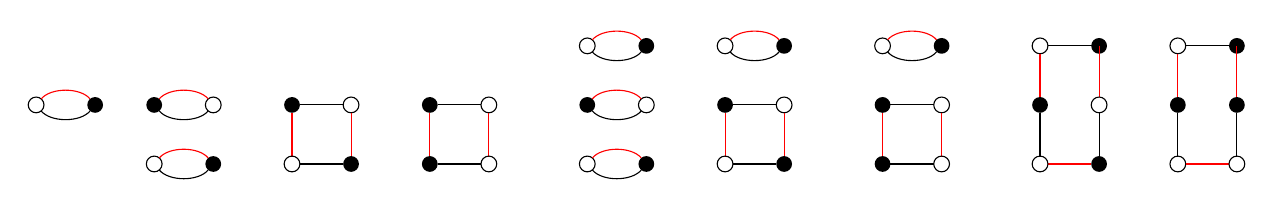
\begin{tikzpicture}[xscale=1,yscale=1]
%%% mono link n=1 
\draw[solid] (0.5,1.5) circle (0.1);
\draw[shorten <= 0.1cm, shorten >= 0.1cm](0.5,1.5)  to[out=-50, in=-130]  (1.25,1.5);
\draw[shorten <= 0.1cm, shorten >= 0.1cm, red] (0.5,1.5) to[out=50, in=130]  (1.25,1.5);
\fill[fill=black] (1.25,1.5) circle (0.1);
%%%
%% disconnected n=2 quartic
%%%
\fill[fill=black] (2.5-0.5,1.5) circle (0.1);
\draw[solid] (3.25-0.5,1.5) circle (0.1);
\draw[shorten <= 0.1cm, shorten >= 0.1cm] (2.5-0.5,1.5) to[out=-50, in=-130] (3.25-0.5,1.5);
\draw[shorten <= 0.1cm, shorten >= 0.1cm, red] (2.5-0.5,1.5) to[out=50, in=130] (3.25-0.5,1.5);
\fill[fill=black] (3.25-0.5,0.75) circle (0.1);
\draw[solid] (2.5-0.5,0.75)  circle (0.1);
\draw[shorten <= 0.1cm, shorten >= 0.1cm] (2.5-0.5,0.75)  to[out=-50, in=-130](3.25-0.5,0.75) ;
\draw[shorten <= 0.1cm, shorten >= 0.1cm, red] (2.5-0.5,0.75) to[out=50, in=130] (3.25-0.5,0.75);
%%% 
%% bipartite unitary quartic n=2 
%%%% 
\fill[fill=black] (4.5-0.75,1.5) circle (0.1);
\draw (4.6-0.75,1.5) -- (5.15-0.75,1.5); 
\draw[solid] (5.25-0.75,1.5) circle (0.1);
\draw [red] (4.5-0.75,1.4) -- (4.5-0.75,0.84); 
\draw [red] (5.25-0.75,1.4) -- (5.25-0.75,0.84); 
\fill[fill=black] (5.25-0.75,0.75) circle (0.1);
\draw (4.6-0.75,0.75) -- (5.15-0.75,0.75); 
\draw[solid] (4.5-0.75,0.75)  circle (0.1);
%%% 
%% Non-bipartite one 
\fill[fill=black] (6.5-1,1.5) circle (0.1);
\draw (6.6-1,1.5) -- (7.15-1,1.5); 
\draw[solid] (7.25-1,1.5) circle (0.1);
%%%
\draw [red]  (6.5-1,1.4) -- (6.5-1,0.84); 
\draw [red]  (7.25-1,1.4) -- (7.25-1,0.84); 
%% 
\fill[fill=black] (6.5-1,0.75) circle (0.1);
\draw  (6.6-1,0.75) -- (7.15-1,0.75); 
\draw[solid] (7.25-1,0.75)   circle (0.1);
%%% 
%% n=3 totally disconnected
\draw[solid] (8.5-1,2.25) circle (0.1);
\draw[shorten <= 0.1cm, shorten >= 0.1cm](8.5-1,2.25)  to[out=-50, in=-130]  (9.25-1,2.25);
\draw[shorten <= 0.1cm, shorten >= 0.1cm, red] (8.5-1,2.25) to[out=50, in=130]  (9.25-1,2.25);
\fill[fill=black] (9.25-1,2.25) circle (0.1);
%% disconnected 
\fill[fill=black] (8.5-1,1.5) circle (0.1);
\draw[solid] (9.25-1,1.5) circle (0.1);
\draw[shorten <= 0.1cm, shorten >= 0.1cm] (8.5-1,1.5) to[out=-50, in=-130] (9.25-1,1.5);
\draw[shorten <= 0.1cm, shorten >= 0.1cm, red] (8.5-1,1.5) to[out=50, in=130] (9.25-1,1.5);
\fill[fill=black] (9.25-1,0.75) circle (0.1);
\draw[solid] (8.5-1,0.75)  circle (0.1);
\draw[shorten <= 0.1cm, shorten >= 0.1cm] (8.5-1,0.75)  to[out=-50, in=-130](9.25-1,0.75) ;
\draw[shorten <= 0.1cm, shorten >= 0.1cm, red] (8.5-1,0.75) to[out=50, in=130] (9.25-1,0.75);
%%% 
%%% %% n=3 2+4 disconnected
\draw[solid] (10.5-1.25,2.25) circle (0.1);
\draw[shorten <= 0.1cm, shorten >= 0.1cm](10.5-1.25,2.25)  to[out=-50, in=-130]  (11.25-1.25,2.25);
\draw[shorten <= 0.1cm, shorten >= 0.1cm, red] (10.5-1.25,2.25) to[out=50, in=130]  (11.25-1.25,2.25);
\fill[fill=black] (11.25-1.25,2.25) circle (0.1);
%% + bipartite sector
\fill[fill=black] (10.5-1.25,1.5) circle (0.1);
\draw (10.6-1.25,1.5) -- (11.15-1.25,1.5); 
\draw[solid] (11.25-1.25,1.5) circle (0.1);
\draw [red] (10.5-1.25,1.4) -- (10.5-1.25,0.84); 
\draw [red] (11.25-1.25,1.4) -- (11.25-1.25,0.84); 
\fill[fill=black] (11.25-1.25,0.75) circle (0.1);
\draw (10.6-1.25,0.75) -- (11.15-1.25,0.75); 
\draw[solid] (10.5-1.25,0.75)  circle (0.1);
%%% 
%%% %% n=3 2+4 disconnected non bipartite
\draw[solid] (12.5-1.25,2.25) circle (0.1);
\draw[shorten <= 0.1cm, shorten >= 0.1cm](12.5-1.25,2.25)  to[out=-50, in=-130]  (13.25-1.25,2.25);
\draw[shorten <= 0.1cm, shorten >= 0.1cm, red] (12.5-1.25,2.25) to[out=50, in=130]  (13.25-1.25,2.25);
\fill[fill=black] (13.25-1.25,2.25) circle (0.1);
%% + non bipartite sector
\fill[fill=black] (12.5-1.25,1.5) circle (0.1);
\draw (12.6-1.25,1.5) -- (13.15-1.25,1.5); 
\draw[solid] (13.25-1.25,1.5) circle (0.1);
\draw [red] (12.5-1.25,1.4) -- (12.5-1.25,0.84); 
\draw [red] (13.25-1.25,1.4) -- (13.25-1.25,0.84); 
\fill[fill=black] (12.5-1.25,0.75)  circle (0.1);
\draw (12.6-1.25,0.75) -- (13.15-1.25,0.75); 
\draw[solid] (13.25-1.25,0.75)  circle (0.1); 
%% 
%% Cycle bi-partite n = 3 
%%% 
\draw[solid] (14.5-1.25,2.25) circle (0.1);
\draw (14.6-1.25,2.25) -- (15.25-1.25,2.25); 
\fill[fill=black] (15.25-1.25,2.25) circle (0.1);
\draw[red] (15.25-1.25,2.25) -- (15.25-1.25,1.6);
\fill[fill=black] (14.5-1.25,1.5) circle (0.1);
\draw[solid] (15.25-1.25,1.5) circle (0.1);
\draw  (15.25-1.25,1.4) -- (15.25-1.25,0.84); 
\fill[fill=black] (15.25-1.25,0.75) circle (0.1);
\draw [red](14.6-1.25,0.75) -- (15.15-1.25,0.75); 
\draw  (14.5-1.25,1.4) -- (14.5-1.25,0.84); 
\draw[solid] (14.5-1.25,0.75)  circle (0.1); 
\draw [red] (14.5 - 1.25,1.6) -- (14.5 - 1.25,2.15); 
%%% 
\draw[solid] (16.0-1,2.25) circle (0.1);
\draw (16.1-1,2.25) -- (16.75-1,2.25); 
\fill[fill=black] (16.75-1,2.25) circle (0.1);
\draw[red] (16.75-1,2.25) -- (16.75-1,1.6);
\fill[fill=black] (16.0-1,1.5) circle (0.1);
\fill[fill=black] (16.75-1,1.5) circle (0.1);
\draw  (16.75-1,1.4) -- (16.75-1,0.84); 
\draw[solid] (16.0-1,0.75)  circle (0.1);
\draw [red](16.1-1,0.75) -- (16.65-1,0.75); 
\draw  (16.0-1,1.4) -- (16.0-1,0.84); 
\draw[solid] (16.75-1,0.75) circle (0.1); 
\draw [red] (16.0-1,1.6) -- (16.0-1,2.15); 
%%% 
\end{tikzpicture}

\end{document}